\documentclass[tikz,border=2pt]{standalone}
\usepackage{amsmath}
\usepackage{tikz}
\usepackage{helvet}
\renewcommand{\familydefault}{\sfdefault}
\usetikzlibrary{arrows.meta, positioning, fit, backgrounds, shapes.geometric, calc}

\definecolor{bandA}{HTML}{440154}
\definecolor{bandB}{HTML}{3B528B}
\definecolor{bandC}{HTML}{21918C}
\definecolor{bandD}{HTML}{5EC962}
\definecolor{bandE}{HTML}{FDE725}
\definecolor{pooledgrey}{HTML}{555555}
\definecolor{panelbg}{HTML}{F5F5F5}
\definecolor{panelline}{HTML}{9A9A9A}
\definecolor{fusionblue}{HTML}{2E5EAA}

\begin{document}
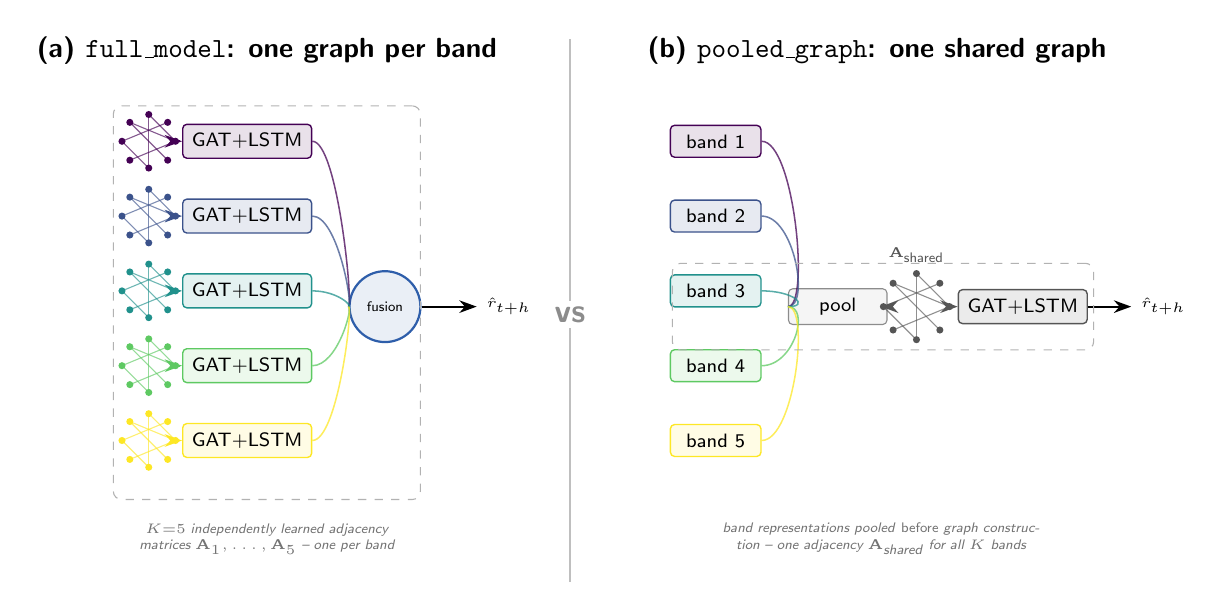
\begin{tikzpicture}[
    font=\sffamily\footnotesize,
    >={Stealth[length=2.2mm,width=1.6mm]},
    every node/.style={align=center},
    panel/.style={draw=panelline, rounded corners=2pt, fill=panelbg, line width=0.5pt},
    modblock/.style={draw=black!55, rounded corners=1.5pt, fill=white, minimum width=1.0cm, minimum height=0.4cm, font=\sffamily\scriptsize, line width=0.5pt},
    titlestyle/.style={font=\sffamily\bfseries\normalsize},
]

\newcommand{\graphicon}[2]{%
    \begin{scope}
        \foreach \a in {0,45,...,315} {\coordinate (gn-\a) at (\a:#2);}
        \draw[#1, line width=0.4pt, opacity=0.65] (gn-0) -- (gn-90);
        \draw[#1, line width=0.4pt, opacity=0.65] (gn-0) -- (gn-135);
        \draw[#1, line width=0.4pt, opacity=0.65] (gn-45) -- (gn-180);
        \draw[#1, line width=0.4pt, opacity=0.65] (gn-90) -- (gn-270);
        \draw[#1, line width=0.4pt, opacity=0.65] (gn-135) -- (gn-315);
        \draw[#1, line width=0.4pt, opacity=0.65] (gn-180) -- (gn-270);
        \draw[#1, line width=0.4pt, opacity=0.65] (gn-225) -- (gn-0);
        \foreach \a in {0,45,...,315} {\fill[#1] (gn-\a) circle (0.045);}
    \end{scope}
}

% ================= LEFT PANEL: full_model (per-band graphs) =================
\node[titlestyle, anchor=south] at (2.0,5.05) {(a) \texttt{full\_model}: one graph per band};

\coordinate (Lstart) at (0,0);
\foreach \i/\col in {0/bandA, 1/bandB, 2/bandC, 3/bandD, 4/bandE} {
    \pgfmathsetmacro{\yy}{4.2 - \i*0.95}
    \begin{scope}[shift={($(Lstart)+(0.5,\yy)$)}]
        \graphicon{\col}{0.34}
    \end{scope}
    \node[modblock, fill=\col!12, draw=\col, minimum width=1.5cm] (gl\i) at ($(Lstart)+(1.75,\yy)$) {GAT+LSTM};
    \draw[->, \col, line width=0.6pt] ($(Lstart)+(0.9,\yy)$) -- (gl\i.west);
}
\node[fill=fusionblue!10, draw=fusionblue, circle, minimum size=0.9cm, line width=0.8pt, font=\sffamily\tiny] (Lfusion) at ($(Lstart)+(3.5,2.1)$) {fusion};
\foreach \i/\col in {0/bandA, 1/bandB, 2/bandC, 3/bandD, 4/bandE} {
    \pgfmathsetmacro{\yy}{4.2 - \i*0.95}
    \draw[\col, line width=0.55pt, opacity=0.75] (gl\i.east) .. controls ($(Lstart)+(2.9,\yy)$) and ($(Lstart)+(3.1,2.1)$) .. (Lfusion.west);
}
\draw[->, line width=0.7pt] (Lfusion.east) -- ++(0.7,0) node[right, font=\sffamily\tiny] {$\hat r_{t+h}$};

\coordinate (LboxBL) at ($(Lstart)+(0.05,-0.35)$);
\coordinate (LboxTR) at ($(Lstart)+(3.95,4.65)$);
\node[draw=black!30, dashed, rounded corners=3pt, fit=(LboxBL) (LboxTR), inner sep=0pt] {};
\node[font=\sffamily\tiny\itshape, black!55, text width=4.4cm] at (2.0,-0.85) {$K{=}5$ independently learned adjacency matrices $\mathbf{A}_1,\ldots,\mathbf{A}_5$ -- one per band};

% ================= DIVIDER =================
\draw[black!25, line width=0.6pt] (5.85,-1.4) -- (5.85,5.5);
\node[font=\sffamily\bfseries\large, black!45, fill=white, inner sep=2pt] at (5.85,2.0) {vs};

% ================= RIGHT PANEL: pooled_graph =================
\node[titlestyle, anchor=south] at (9.75,5.05) {(b) \texttt{pooled\_graph}: one shared graph};

\coordinate (Rstart) at (7.1,0);
\foreach \i/\col in {0/bandA, 1/bandB, 2/bandC, 3/bandD, 4/bandE} {
    \pgfmathsetmacro{\yy}{4.2 - \i*0.95}
    \pgfmathtruncatemacro{\kk}{\i+1}
    \node[modblock, fill=\col!12, draw=\col, minimum width=1.15cm] (rin\i) at ($(Rstart)+(0.6,\yy)$) {band \kk};
}
\node[draw=black!45, rounded corners=1.5pt, fill=black!4, minimum width=1.25cm, minimum height=0.4cm, font=\sffamily\scriptsize] (pool) at ($(Rstart)+(2.15,2.1)$) {pool};
\foreach \i/\col in {0/bandA, 1/bandB, 2/bandC, 3/bandD, 4/bandE} {
    \pgfmathsetmacro{\yy}{4.2 - \i*0.95}
    \draw[\col, line width=0.55pt, opacity=0.75] (rin\i.east) .. controls ($(Rstart)+(1.6,\yy)$) and ($(Rstart)+(1.8,2.1)$) .. (pool.west);
}
\begin{scope}[shift={($(Rstart)+(3.15,2.1)$)}]
    \graphicon{pooledgrey}{0.42}
\end{scope}
\node[font=\sffamily\tiny, pooledgrey] at ($(Rstart)+(3.15,2.75)$) {$\mathbf{A}_{\text{shared}}$};
\draw[->, pooledgrey, line width=0.7pt] (pool.east) -- ($(Rstart)+(2.7,2.1)$);

\node[modblock, fill=pooledgrey!12, draw=pooledgrey, minimum width=1.6cm] (rgat) at ($(Rstart)+(4.5,2.1)$) {GAT+LSTM};
\draw[->, pooledgrey, line width=0.7pt] ($(Rstart)+(3.6,2.1)$) -- (rgat.west);
\draw[->, line width=0.7pt] (rgat.east) -- ++(0.55,0) node[right, font=\sffamily\tiny] {$\hat r_{t+h}$};

\coordinate (RboxBL) at ($(Rstart)+(0.05,1.55)$);
\coordinate (RboxTR) at ($(Rstart)+(5.4,2.65)$);
\node[draw=black!30, dashed, rounded corners=3pt, fit=(RboxBL) (RboxTR), inner sep=0pt] {};
\node[font=\sffamily\tiny\itshape, black!55, text width=5.8cm] at ($(Rstart)+(2.7,-0.85)$) {band representations pooled \emph{before} graph construction -- one adjacency $\mathbf{A}_{\text{shared}}$ for all $K$ bands};

\end{tikzpicture}
\end{document}
